% 
% Annual Cognitive Science Conference
% Sample LaTeX Paper -- Proceedings Format
% 

% Original : Ashwin Ram (ashwin@cc.gatech.edu)       04/01/1994
% Modified : Johanna Moore (jmoore@cs.pitt.edu)      03/17/1995
% Modified : David Noelle (noelle@ucsd.edu)          03/15/1996
% Modified : Pat Langley (langley@cs.stanford.edu)   01/26/1997
% Latex2e corrections by Ramin Charles Nakisa        01/28/1997 
% Modified : Tina Eliassi-Rad (eliassi@cs.wisc.edu)  01/31/1998
% Modified : Trisha Yannuzzi (trisha@ircs.upenn.edu) 12/28/1999 (in process)
% Modified : Mary Ellen Foster (M.E.Foster@ed.ac.uk) 12/11/2000
% Modified : Ken Forbus                              01/23/2004
% Modified : Eli M. Silk (esilk@pitt.edu)            05/24/2005
% Modified : Niels Taatgen (taatgen@cmu.edu)         10/24/2006
% Modified : David Noelle (dnoelle@ucmerced.edu)     11/19/2014

%% Change "letterpaper" in the following line to "a4paper" if you must.

\documentclass[10pt,letterpaper]{article}

\usepackage{cogsci}
\usepackage{pslatex}
\usepackage{apacite}
\usepackage{graphicx}

\title{Morphosyntactic and Referential Cues to the Identification of Generic Statements}
 
\author{{\large \bf Phil Crone} \\
	\texttt{pcrone@stanford.edu}\\
  Department of Linguistics \\
  Stanford University
  \And {\large \bf Michael C. Frank} \\
  \texttt{mcfrank@stanford.edu}\\
  Department of Psychology \\
  Stanford University}

\begin{document}

\maketitle

\begin{abstract}
Generic sentences (e.g., ``birds lay eggs'') express generalizations about kinds, as opposed specific individuals or groups of individuals (e.g., ``all birds lay eggs''). Generics are an important method of transmitting cultural knowledge, but because there is no unique marker of genericity, identifying whether a sentence is generic is a challenge. Here we investigated how language users use morphosyntactic and pragmatic cues to determine whether naturalistic sentences should receive generic interpretations. Experiment 1 demonstrates the effect of the morphosyntactic features of a sentence's subject noun phrase (NP) on generic interpretation. Experiments 2 and 3 reveal that when a sentence's subject NP does not have an obvious reference in context, the sentence is more likely to receive a generic interpretation. These data suggest the beginnings of an account by which cues to genericity could be combined to make graded, contextual judgments about whether an utterance has an intended generic meaning.

\textbf{Keywords:} Psycholinguistics; pragmatics; generics.
\end{abstract}


\section{Introduction}
 % 3x puzzle

% importance of generics
% propopositional definition can be rephrased
% lay eggs is a good example
% "while much research has been focused on problem 1"

Generic sentences express generalizations about kinds rather than individuals and are an important route for the transmission of cultural knowledge \cite{gelman2003}. For example, the sentence ``birds lay eggs'' expresses a general property of the kind \textit{bird}, whereas ``all birds lay eggs'' means that every member of the set lays eggs. A key difference between generic and non-generic statements is that generics allow for exceptions: ``birds lay eggs'' is true despite the fact that at least half of birds do not. In contrast, ``all birds lay eggs'' is technically false, because male birds don't \cite{Prasada:2000}. 

Generics are not consistently marked by any particular lexical, morphological, or syntactic convention, so how do we know that a sentence is generic? Prior work suggest that we use at least three types of cues to guide the interpretation of sentences as generic or non-generic: morphosyntactic features, pragmatic cues, and world knowledge. In English, the subject noun phase (NP) of a generic sentence is often a bare plural (``birds fly''), but can also be an indefinite singular (``a bird has wings'') and definite singular (``the bird is a warm-blooded animal''). In contrast, definite plural NPs (``the birds have feathers'') are generally thought to force non-generic interpretations. Tense and aspect also cue whether a sentence is interpreted generically; simple present tense (``birds fly'') is typically more generic than e.g., present progressive (``birds are flying overhead'') or past (``birds flew past my window'') \cite{Carlson:1977,Krifka:1995,Lyons:1977}. 

Pragmatics and world knowledge can also influence whether a sentence is interpreted as generic or non-generic. For example, if a unique bird is present in the context of an utterance of a sentence with the subject NP ``the bird,'' this NP is likely to be interpreted as non-generic and as referring to the bird in context. Conversely, if no such bird exists in the context, a generic interpretation may be preferred. Finally, world knowledge about properties shared by members of a kind influences the interpretation of potentially generic sentences. The sentence ``a bird does not fly'' is interpreted as being about some particular bird (e.g., a penguin), given world knowledge that, in general, birds fly. 

Previous experimental work has confirmed the influence of these three types of factors on children's and adults' identification of generics. Adults and children as young as 3 show a preference for interpreting bare plurals as generic, as compared to definite plurals, and prefer generic interpretations when the subject NP has no available referent in context \cite{Gelman:2003}. By age 3, children are less likely to assign a generic interpretation to a sentence when its subject NP has a possible referent in the preceding linguistic context, and they can also use knowledge about whether properties are generalizable to kinds as evidence about genericity  \cite{Cimpian:2008}. Young children can also use the definiteness of subject NPs, as well as tense and aspect, in this process \cite{Cimpian:2011}.

The present study builds on previous work in two ways. First, we focus on the quantitative relationship between factors in adults' recognition of generics. Most previous work on the identification of generics has focused on children's abilities, perhaps stemming in part from an assumption that children face challenges in identifying generics that are less relevant for adults. However, work emphasizing the probabilistic nature of language comprehension suggests that adults face a similar problem \cite{Levy:2008,Frank:2012}. On this view, language users resolve uncertainty in comprehension via probabilistic inference to the most likely interpretation. In the case of identifying generics, we can take adults to reason about the likelihood that an utterance is generic given morphosyntactic features of the sentence, features of the context, and the their own world knowledge. Second, we collect naturalistic examples of generic and non-generic sentences generated by study participants, allowing for a more realistic representation of how genericity is used in natural language. 

Our plan is as follows. We begin by introducing an experimental paradigm that allows us to measure the relative genericity of the statements that participants produce; we use this paradigm to examine the role of morphosyntactic information in genericity (Experiment 1). We next investigate the interaction between morphosyntactic information and pragmatic information about reference (Experiments 2A and B). Finally, we identify a set of sentences whose genericity is ambiguous and demonstrate the independence of morphosyntactic and pragmatic information (Experiment 3). Taken together, these experiments indicate that morphosyntactic and pragmatic cues are separable parts of fundamentally graded inferences about whether sentences refer to individuals or kinds. 
% The approach also allows for consideration of examples that are more ambiguous between generic and non-generic interpretations than examples created by experimenters. 

\section{Experiment 1: Morphosyntactic Cues}

As discussed above, the number and definiteness of a sentence's subject NP influence its interpretation as generic or non-generic \cite{Carlson:1977,Krifka:1995,Lyons:1977}. Previous work investigating morphosyntactic cues to genericity have fixed the number of the subject NP as either singular \cite{Cimpian:2011} or plural \cite{Gelman:2003} and only manipulated definiteness. In Experiment 1, we considered the effects of number, definiteness, and their interaction on the interpretation of generics. Participants performed a sentence completion task in which the subject NP was provided. They then indicated whether the sentences they produced were about specific individuals or kinds.

\subsection{Method}

\subsubsection{Participants} 

We recruited 100 participants to participate through Amazon's Mechanical Turk website. We restricted participants to individuals within the United States and paid them 50 cents to complete the study. The study took approximately 14 minutes to complete. We excluded 4 participants for indicating that their native language was not English.

\subsubsection{Stimuli}  

Forty-eight nouns were chosen to use as the bases for subject NPs. To ensure diversity among these subject NPs, twenty-four nouns were animate and twenty-four were inanimate. For each participant, each noun was randomly assigned morphosyntactic features using a \(2 \times 2\) factorial design crossing number (singular, plural) with definiteness (definite, indefinite). Half of nouns assigned to each factorial point were animate and half were inanimate. We then edited the nouns to reflect the assigned number and definiteness values and create full NPs. For example, if the noun ``panda'' were assigned values \textit{plural} and \textit{definite}, the full NP would be ``the pandas.''

In the first part of the experiment, participants saw a single NP followed by a single-line text box. They were instructed to ``write a sentence starting with the phrase below.'' In the second part of the experiment, participants were shown the sentences they had written in the first part of the experiment. They viewed one sentence at a time and asked whether the sentence was about a specific \textit{noun} (for singular NPs), a specific group of \textit{nouns} (for plural NPs), or about \textit{nouns} in general. Participants indicated their response using a 5-point Likert scale with the following values: ``Definitely about a specific \textit{noun}/group of \textit{nouns} (=1),'' ``Probably about a specific \textit{noun}/group of \textit{nouns},'' ``Not sure,'' ``Probably about \textit{nouns} in general,'' ``Definitely about \textit{nouns} in general (=5).''

\subsubsection{Procedure} 

We first presented participants with four example NPs. After providing sentence completions for these items, participants were shown an example sentence completion for the NP. These sentences were constructed to favor non-generic interpretations for all NP types. After seeing the examples, participants were informed that they would not receive any feedback for the rest of the experiment.

Participants then began the first part of the experiment. All forty-eight subject NPs were presented in pseudorandom order, counterbalanced so that no two consecutive NPs matched in both number and definiteness. We required participants to provide a sentence completion at least six characters in length for each item. After completing part 1, participants entered the second part of the experiment and were informed that they would be evaluating sentences' genericity. They evaluated the sentences they had produced in part 1 in the manner described above. Sentences were again presented in a pseudorandom order counterbalanced so that no two consecutive NPs matched in both number and definiteness. After judging all forty-eight sentences, participants were required to report their native language. We measured reaction times for each item, measured from the time the item was presented until the time a response was submitted. In the second part of the experiment, we excluded responses whose reaction times were greater than 2 standard deviations from the mean.

% \subsubsection{Data Analysis} 


\begin{table*}
\begin{center} 
\caption{Example Productions from Experiment 1. Generic sentences received ratings of 5; non-generics received ratings of 1.} 
\label{tab:ex} 
\vskip 0.12in
\begin{tabular}{cccc} 
\hline
Definiteness    &  Number & Genericity & Examples \\
\hline
Indefinite        &   Singular & Generic & ``A cow eats grass.'', ``A bicycle is a convenient form of transportation.''\\
Indefinite  &   Singular & Non-generic & ``A dog is sleeping on the porch.'', ``A light bulb was dropped and exploded.''\\
Indefinite           &   Plural & Generic & ``Gorillas are primates.'', ``Towels are useful after showering.''\\
Indefinite         &   Plural  & Non-generic & ``Cats are circling the fishtank.'', ``Kites were flying at the beach.''\\
Definite        &   Singular & Generic & ``The camel uses his humps to conserve water.'', ``The clock tells time.''  \\
Definite  &   Singular & Non-generic & ``The bear is moving closer to us.'', ``The bed is unmade.''\\
Definite           &   Plural & Generic & ``The kangaroos carry babies in pouches.'', ``The trumpets are loud.'' \\
Definite         &   Plural & Non-generic & ``The rabbits are digging holes in the yard.'', ``The couches were dusty and old.''\\
\hline
\end{tabular} 
\end{center} 
\end{table*}

\subsection{Results and Discussion}

We found that both definiteness and number affected mean genericity ratings (Figure \ref{fig:e1}). The definites that participants produced tended to be rated as less generic, while indefinites---especially ``bare plural'' indefinites---tended to be rated as more generic (see Table \ref{tab:ex} for examples).

\begin{figure}[t]
\centering
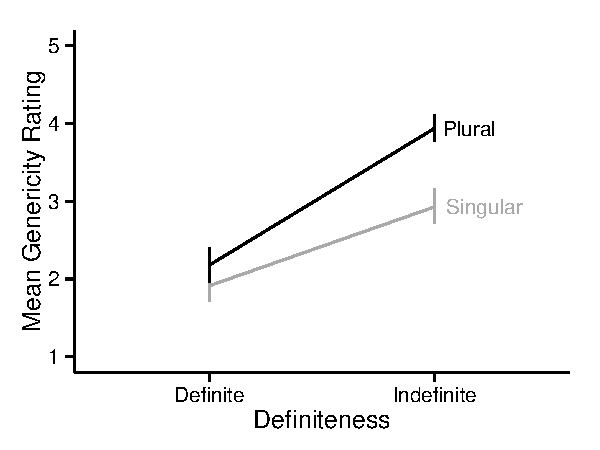
\includegraphics[width=.9\linewidth]{figures/e1.pdf}
\caption{\label{fig:e1} Mean genericity ratings in Experiment 1 by definiteness and number. Error bars show 95\% confidence intervals.} 
\end{figure}

To analyze the results, we fit a linear mixed-effects model to predict participants' genericity ratings. We examined the interaction between animacy, definiteness, and number of subject NPs.\footnote{Mixed-effects models were fit in R v. 3.1.2 using the lme4 package. The model specification was as follows: \texttt{response} \(\sim\) \texttt{animacy * definiteness * number + (animacy + definiteness + number | WorkerId) + (definiteness + number | subject NP)}. We calculated \(p\) values by treating the \(t\) statistic as if it were a \(z\) statistic \cite{Barr:2013}.} The model shows main effects of animacy, definiteness, and number. Sentences with indefinite NP subjects were rated significantly more generic (\(\beta = 1.745, t = 14.169, p < 0.001\)). Sentences with singular NP subjects (\(\beta = -0.302, t = -3.450, p < 0.001\)), and inanimate subjects (\(\beta = -0.503, t = -5.732, p < 0.001\)), were rated less generic. In addition, the model revealed an interaction effect between definiteness and number such that indefinite singulars were rated significantly less generic (\(\beta = -1.023, t = -9.913, p < 0.001\)). Finally, there was a significant three-way interaction such that inanimate, indefinite singulars were rated significantly more generic (\(\beta = 0.536, t = 3.669, p < 0.001\)). 

The results are consistent with previous findings that indefinite singulars and bare plurals facilitate generic interpretations compared to definite singulars and definite plurals, respectively \cite{Cimpian:2011, Gelman:2003}. However, these results also show that plurality is independently associated with genericity, which has not been previously acknowledged. The interaction between definiteness and plurality reveals a superadditive effect by which indefinite singulars support generic interpretation less than bare plurals. This is unsurprising, as bare plurals are often taken to be the canonical subject type for English generics \cite{Carlson:1977,Krifka:1995,Lyons:1977}. The effect of animacy is consistent with previous findings that both children and adults produce more generic statements in describing animals than in describing artifacts \cite{Brandone:2009}.

The most unexpected finding is that definite plurals were rated more generic overall than definite singulars, despite the general view that definite singulars, but not definite plurals, allow for generic interpretations in English. This result forced us consider whether our methodology measured some property other than genericity. However, inspection of definite plurals that received high genericity ratings suggested that these ratings were at least \emph{prima facie} appropriate.

\section{Experiment 2A: Contextual Cues in Production}

Experiment 1 demonstrated the role of morphosyntactic and, in the case of animacy, world knowledge cues to identifying generic statements. However, this experiment left contextual cues unaddressed. Experiment 2A investigated the role of context as a cue to identifying generics. Specifically, this experiment examined whether language users would be less likely to treat a subject NP as generic when it has a possible referent in the context.

\subsection{Method}

\subsubsection{Participants} 

Recruitment details were identical to Experiment 1; we excluded two participants whose native languages were not English for a final sample of 98 participants.

\subsubsection{Stimuli} 

Stimuli were nearly identical to those in Experiment 1. However, in part 1 of the experiment, each item was presented with an image depicting either one or five instances of the animal or artifact denoted by the subject NP (Figure \ref{fig:stim}). Images with only one instance were taken directly from the Bank of Standardized Stimuli v. 2.0 \cite{Brodeur:2014}. Images with multiple instances of the animal or artifact were created from the single instance images. The number of individuals in the image either matched or mismatched the number of the subject NP. Half of items for each NP type were paired with matching images and half were paired with mismatching images. Participants were instructed to describe the image in their sentence completion. The images only appeared for the sentence completion portion of the experiment; they did not appear in the rating portion.

\subsubsection{Procedure} 

The procedure was identical to that of Experiment 1. For the four example items, two items were randomly chosen to have matching images, the other items had mismatching images.
 % As in Experiment 1, the order of items in both parts of the experiment were pseudorandomized with counterbalancing to ensure that no two consecutive items used subject NPs with the same number and definiteness features. The order of images was not controlled.

% \subsubsection{Data Analysis} \quad. Thus, responses from 98 participants were analyzed. In addition, responses from items whose reaction times were greater than 2 standard deviations from the mean for the second part of the experiment were excluded from the analysis.

\begin{figure}[t]
\begin{center}
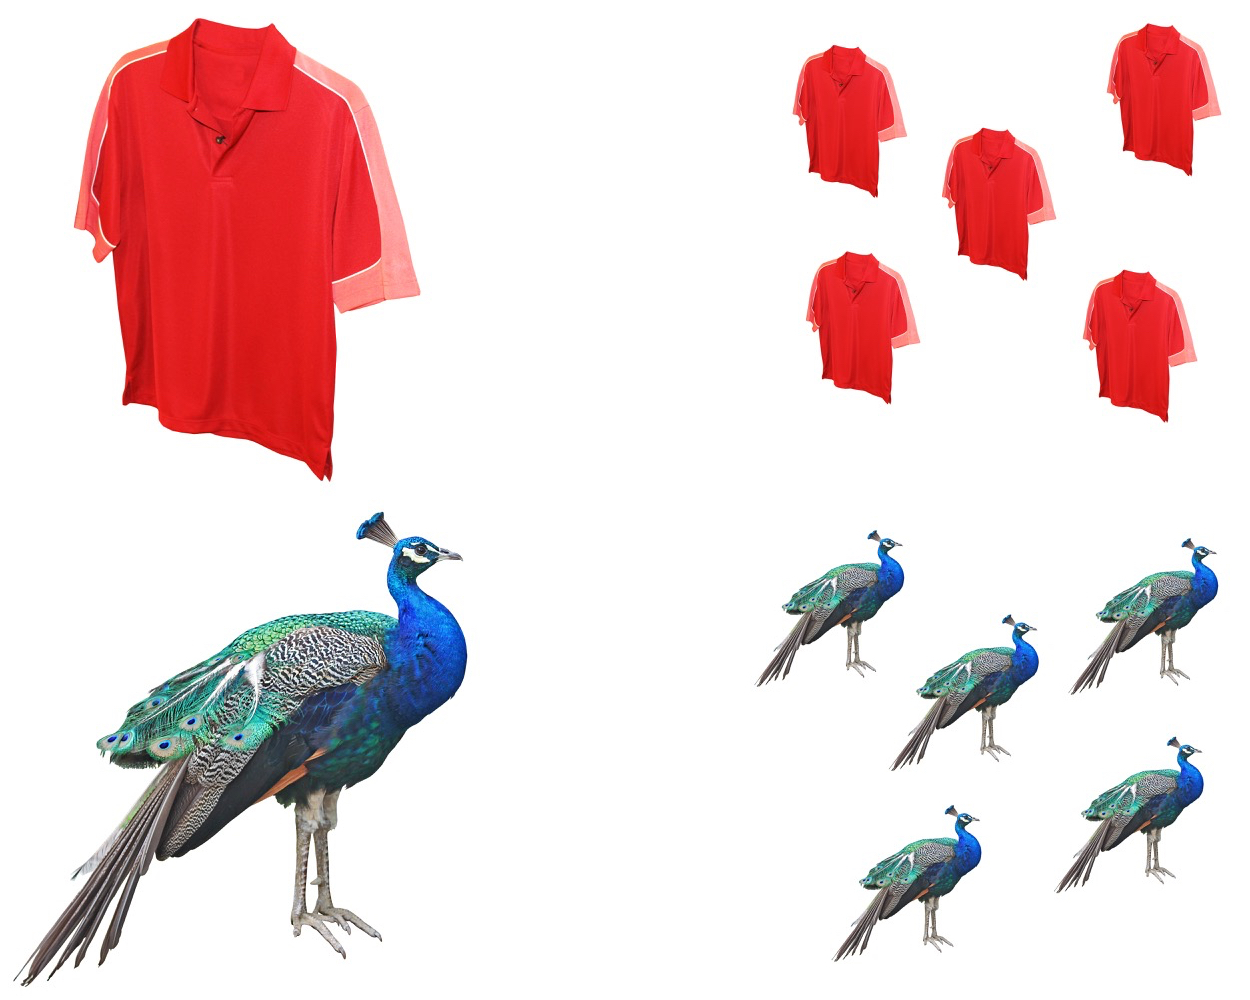
\includegraphics[width=0.3\textwidth]{figures/stimuli.jpg}
\end{center}
\caption{Examples of images used in Experiments 2A, 2B, and 3. Clockwise from upper left: single shirt, multiple shirts, multiple peacocks, single peacock.} 
\label{fig:stim}
\end{figure}

\subsection{Results and Discussion}

\begin{figure}[t]
\centering
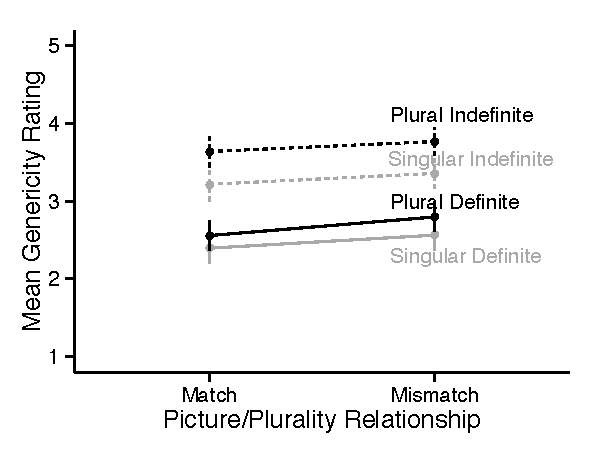
\includegraphics[width=.9\linewidth]{figures/e2a_mod.pdf}
\caption{\label{fig:e2a} Mean genericity ratings from Experiment 2A (ratings by producers), plotted by picture/plurality match/mismatch, definiteness, and number. Error bars show 95\% confidence intervals.} 
\end{figure}

Genericity ratings are shown in Figure \ref{fig:e2a}. We replicated the morphosyntactic effects in Experiment 1. In addition, there was a small but reliable effect of referential mismatch such that sentences generated to refer to a picture that mismatched their base NP in number were later rated as more generic. 

As in Experiment 1, we fit a linear mixed-effects model to predict participants' genericity ratings. We examined the interaction of animacy, definiteness, and number of the subject NP, as well as image match/mismatch.\footnote{The model specification was as follows: \texttt{response} \(\sim\) \texttt{animacy * definiteness * number * image + (animacy + definiteness + number + image | Worke����rId) + (definiteness + number + image | subject NP)}.} There were significant main effects of animacy, definiteness, and image. Sentences with indefinite subject NPs were rated more generic (\(\beta = 1.023, t = 7.518, p < 0.001\)), while sentences with inanimate subjects were rated less generic (\(\beta = -0.742, t = -4.005, p < 0.001\)). Sentences produced with an image that did not match the subject NP in number were also rated significantly more generic (\(\beta = 0.389, t = 3.414, p < 0.001\)). The model also revealed interaction effects between definiteness and number such that sentences with indefinite singular subjects were significantly less generic (\(\beta = -0.340, t= -2.170, p = 0.03\)), and between definiteness and image such that sentences with indefinite subjects that appears with mismatching images were less generic (\(\beta = -0.426, t = -2.731, p < 0.001\)). Finally, the model showed a significant three-way interaction such that inanimate, indefinite subjects with mismatching images were rated significantly more generic (\(\beta = 0.567, t = 2.571, p = 0.01\)). In general, these effects are similar to those in Experiment 1. 

% Several of these effects are similar to those observed in Experiment 1, and can be interpreted similarly. The main effect of subject NP number that was observed in Experiment 1 did not appear in the model for Experiment 2; the effect of number in the model was in the expected direction, with sentences with singular subjects being rated less generic, but was not significant (\(\beta = -0.162, t = -1.397, p > 0.1\)). 

The most important finding of Experiment 2A was the result that referential mismatch increased genericity. 
% Participants generated more generic sentences when the subject NP did not have a clear referent in the image. This results suggests that language users are sensitive to whether an NP refers in context in producing generics.
This result is similar to the finding of \citeA{Gelman:2003}, who showed that children and adults are more likely to interpret pronouns as generic when the only possible contextual referent mismatches in number. However, Gelman and Raman hypothesized that this effect would only be seen for plural subjects in contexts with only singular referents. In contrast, we observed this (modest) effect in all NP conditions, suggesting that genericity is generally supported when NPs fail to have a reference in context, regardless of the NP's number. Nevertheless, this experiment focused on whether generic sentences are \emph{produced} more often for a given NP when this NP has a contextual referent. This is a slightly different question, however, than whether \emph{listeners} are more likely to interpret sentences as generic when the subject NP fails to refer in context. We investigated this question in Experiment 2B. 

\section{Experiment 2B: Contextual Cues in Comprehension}

\subsection{Method}

\subsubsection{Participants} Recruitment details were as above, except the study took 4 minutes and compensation was 30 cents. We recruited 190 participants, excluding five for non-English native languages; our final sample consisted of 185 participants.

\subsubsection{Stimuli} 

Each participant in Experiment 2B was assigned some set of sentences produced by a specific participant from Experiment 2A. This set consisted of the twenty-four sentences a participant in Experiment 2A produced while viewing a picture that matched the subject NP in number. Each participant in Experiment 2A was matched with two individuals in Experiment 2B. (In addition to the two non-native English speakers from Experiment 2A, three producers were excluded for producing offensive or inappropriate sentences).

Participants were told that other Mechanical Turk workers had produced the sentences they were evaluating as descriptions of the pictures they saw seeing. Stimuli were presented in a manner similar to part 2 of Experiment 2A, but images were displayed above each sentence. Half of the sentences for each NP subject type were presented with an image that matched the subject NP in number, while half were presented with an image that mismatched in number. For each item that was seen with a matching image by one participant, that item was seen with a mismatching image by a second participant. 

\subsubsection{Procedure}

The procedure was the same as that for part 2 of Experiments 1 and 2A. Participants were instructed to pay attention to the images and consider what the other Mechanical Turk worker had in mind when writing each sentence. For the four example items, two items were randomly chosen to have matching images, the other items had mismatching images. 
% Participants did not receive any feedback after providing genericity judgments for the four example items. As in Experiments 1 and 2A, the order of items in both parts of the experiment were pseudorandomized with counterbalancing to ensure that no two consecutive items used subject NPs with the same number and definiteness features. The order of images was not controlled.

% \subsubsection{Data Analysis} \quad. In addition, responses from items whose reaction times were greater than 2 standard deviations from the mean were excluded from the analysis.

\subsection{Results and Discussion}


\begin{figure}[t]
\centering
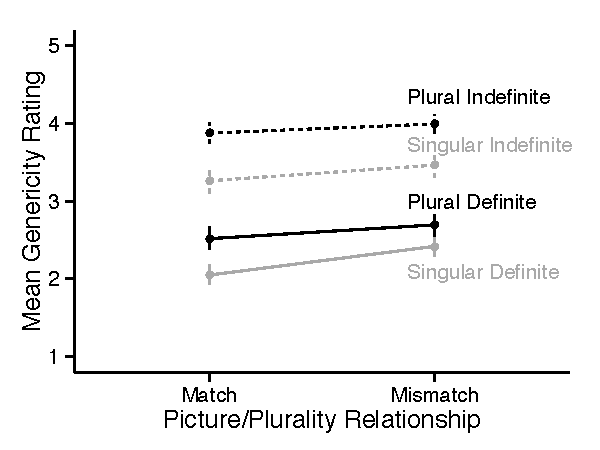
\includegraphics[width=.9\linewidth]{figures/e2b_mod.pdf}
\caption{\label{fig:e2b} Mean genericity ratings from Experiment 2B (independent ratings), plotted by picture/plurality match/mismatch, definiteness, and number. Error bars show 95\% confidence intervals.} 
\end{figure}

Findings were largely comparable to Experiments 1 and 2A: Participants were more likely to interpret a sentence as generic when its subject NP failed to refer in context (Figure \ref{fig:e2b}). This effect was consistent across all NP types. 

We fit an identical linear model to Experiment 2A. The model revealed significant main effects of definiteness, number, and image. Sentences with indefinite subject NPs were rated more generic (\(\beta = 1.401, t = 11.718, p < 0.001\)), while sentences with singular subjects were rated less generic (\(\beta = -0.421, t = -3.642, p < 0.001\)). Sentences produced with an image that did not match the subject NP in number were rated significantly more generic (\(\beta = 0.382, t = 3.604, p < 0.001\)). The model also revealed interaction effects between between definiteness and image such that sentences with indefinite subjects that appears with mismatching images were less generic (\(\beta = -0.302, t = -2.021, p = 0.043\)) and between animacy and image such that sentences with inanimate subjects and mismatching images were less generic (\(\beta = -0.380, t=-2.508, p=0.012\)). Finally, the model showed a significant three-way interaction such that inanimate, indefinite subjects with mismatching images were rated significantly more generic (\(\beta = 0.431, t = 2.028, p = 0.043\)). 

% The results again largely resemble those of Experiments 1 and 2A. As in Experiment 1, there was a significant effect of the number of the subject. However, unlike Experiments 1 and 2A, we found no significant main effect of animacy for \(p < 0.05\), although inanimates were rated as less generic than animates (\(\beta = -0.280, t = -1.822, p = 0.069\)). As in Experiment 2A, the main finding in Experiment 2B was the effect of the image either matching or mismatching the subject NP in number. We find that 

\section{Experiment 3: Ambiguous Sentences}

Although contextual referent mismatch produced effects in Experiments 2A and 2B, the effect size was relatively small in both cases (\(\beta = 0.389\) for Experiment 2A; \(\beta = 0.382\) for Experiment 2B). We hypothesized that this was possibly due to large numbers of sentences that were unambiguously generic or non-generic. In Experiment 3, we investigated whether this effect would be larger if participants considered more ambiguous sentences. We gathered new ratings for the sentences from Experiment 1, identified the most ambiguous of these sentences, and then performed the same referential mismatch manipulation as we used in Experiment 2. 

\subsection{Method} 

\subsubsection{Participants}

In part 1, we recruited 110 participants through Mechanical Turk for 67 cents and excluded one participant for having a non-English native language for a total sample of 109; in part 2, we recruited 100 participants and paid 20 cents, excluding five for a total sample of 95.

\begin{figure}[t]
\centering
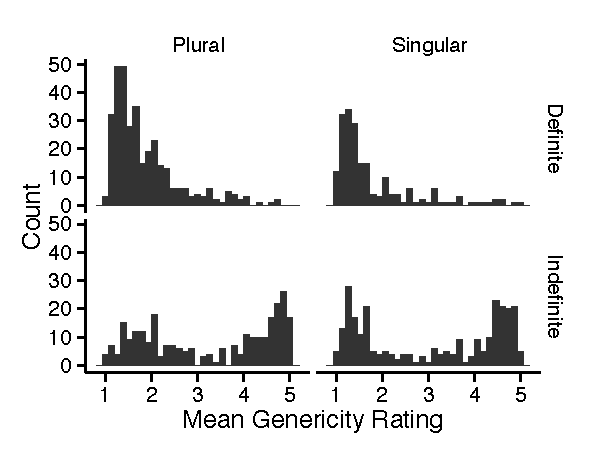
\includegraphics[width=.9\linewidth]{figures/e3_norming_mod.pdf}
\caption{\label{fig:e3norming} Histograms of genericity ratings from the full set of sentences produced for Experiment 3, split by definiteness and number.} 
\end{figure}

\begin{figure}[t]
\centering
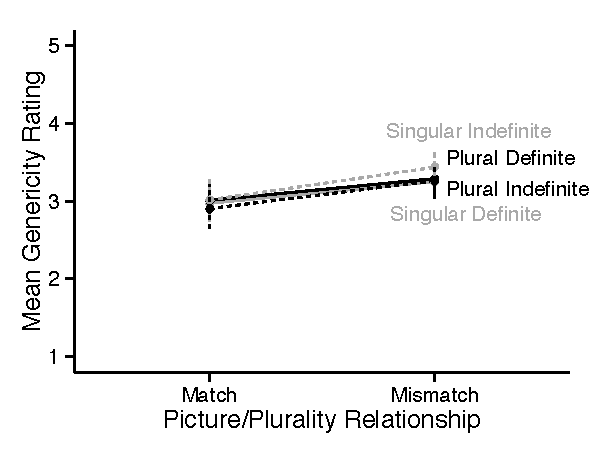
\includegraphics[width=.9\linewidth]{figures/e3_mod.pdf}
\caption{\label{fig:e3} Mean genericity ratings from Experiment 3, plotted by picture/plurality match/mismatch, definiteness, and number. Error bars show 95\% confidence intervals.} 
\end{figure}

\subsubsection{Stimuli}  

Stimuli for the first part of this experiment were drawn from a set of 1100 sentences generated in Experiment 1 that received genericity ratings between 2 and 4, inclusive. We then created 11 non-overlapping subsets, each containing 100 randomly-chosen sentences. This process was repeated to yield 110 sets of 100 sentences each. Since the ambiguous sentences from Experiment 1 were not equally distributed among different NP types, we could not ensure an equal distribution of NP types in these sets. We assigned each participant one set of sentences, displaying them without images as in the genericity judgment portion of Experiment 1.

The stimuli for the second part of this experiment were drawn from those used in the first part. We calculated the mean genericity rating given to each sentence in part 1. We then selected the 20 sentences for each NP type whose mean ratings were closest to 3 and which did not contain any obvious typographical errors. This yielded a set of 80 sentences, which were then divided into groups of 16 sentences with 4 sentences of each NP type. In constructing these sets, animacy was not controlled for; in general, each set contained more animate subjects than inanimate subjects. No set contained multiple sentences with the same subject. These sentences were presented with matching and mismatching images in the same manner as that of Experiment 2B. 

\subsubsection{Procedure} 

In part 1, participants saw four example sentences with feedback, with the definite singular and bare plural example sentences favoring generic interpretations. The target sentences were then presented for rating in randomized order as in the genericity rating portion of Experiment 1. In part 2, the procedure was identical to that of Experiment 2B. 

% \subsubsection{Data Analysis} 

% For calculating the mean ratings for sentences in part one, we excluded 1 participant for indicating that their native language was not English. Thus, responses from 109 participants were analyzed. In addition, responses from items whose reaction times were greater than 2 standard deviations from the mean were excluded. For the second part of the experiment, we excluded 5 participants for indicating that their native language was not English. Thus, responses from 95 participants were analyzed. In addition, responses from items whose reaction times were greater than 2 standard deviations from the mean were excluded.

\subsection{Results and Discussion}

The distribution of mean genericity ratings across sentences is shown in Figure \ref{fig:e3norming}. The majority of definites were not rated as being particularly generic, but the distribution was substantially more bimodal for indefinites. Our procedure resulted in the selection of sentences whose ranking was closest to three; these sentences were relatively rare for all participants.

Turning to the second part of the experiment, we again found a strikingly consistent effect of referential mismatch, though again this effect was small (Figure \ref{fig:e3}). As with the previous experiments, results from the second part of Experiment 3 were analyzed with linear mixed-effects models. We compared two models. The first predicted genericity rating from number, definiteness, image, and their interactions. The second predicted genericity rating from image alone.\footnote{The two model specifications were as follows: \texttt{response} \(\sim\) \texttt{definiteness * number * image + (image | WorkerId)} and \texttt{response} \(\sim\) \texttt{image + (image | WorkerId)}.} There was no significant difference between the fits of the two models (\(\chi^2(6) = 2.738, p = 0.841\)), so we opted for the minimal model, which revealed that sentences presented with mismatching images were rated significantly more generic than those presented with matching images (\(\beta = 0.326, t = 4.192, p < 0.001\)).

\section{General Discussion}

Several of the results found here replicate previous findings about cues to genericity; indefinites are more generic than definites \cite{Cimpian:2011, Gelman:2003}, animates are more generic than inanimates \cite{Brandone:2009}, and lack of a contextual referent supports generic interpretation \cite{Gelman:2003}. However, we have also identified previously unacknowledged cues to genericity. Experiment 1 showed plurality of subject NPs to be a cue to genericity. This is connected to the finding that definite plurals are judged to be more generic than definite singulars, contra standard assumptions about genericity in English. This result suggests that we must broaden our view of which types of English NPs may be kind-denoting.

The results of Experiments 2A, 2B, and 3 show that pragmatic cues regarding contextual referents also play a crucial role in allowing language users to identify generics. Importantly, we observe this effect across all subject NP types. This suggests that there is independent integration of morphosyntactic and pragmatic information about genericity. The view that emerges is one consistent with probabilistic approaches to language comprehension in which language users integrate independent sources of information, both linguistic and non-linguistic, to determine the most likely interpretation. 

\section{Acknowledgments}

Thanks to Daniel Lassiter, Rose Schneider, and the members of the Language and Cognition Lab. We gratefully acknowledge the support of ONR Grant N00014-13-1-0287.

\bibliographystyle{apacite}

\setlength{\bibleftmargin}{.125in}
\setlength{\bibindent}{-\bibleftmargin}

\bibliography{Generics}


\end{document}
